% Field Shift - research paper on the machine-learning models (NASA Space Apps Challenge 2026, Chiclayo, Peru)
% Compile: pdflatex field_shift_ml.tex (twice, for references), or upload paper/field_shift_overleaf.zip to Overleaf.
% Figures are in figures/ (copied from ml/artifacts; v3_overview.png from ml/scripts/paper_v3_figure.py).
\documentclass[11pt,a4paper]{article}

\usepackage[utf8]{inputenc}
\usepackage[T1]{fontenc}
\usepackage{lmodern}
\usepackage[margin=2.3cm]{geometry}
\usepackage{amsmath,amssymb}
\usepackage{graphicx}
\usepackage{booktabs}
\usepackage{tabularx}
\usepackage{array}
\usepackage{float}
\usepackage[font=small,labelfont=bf]{caption}
\usepackage{xcolor}
\usepackage{enumitem}
\usepackage[round]{natbib}
\usepackage[hidelinks]{hyperref}

\newcommand{\sm}{\ensuremath{\mathrm{m^3\,m^{-3}}}}
\newcommand{\ci}[2]{\ensuremath{[#1,\,#2]}}
\setlist{nosep,leftmargin=*}
\renewcommand{\arraystretch}{1.15}

\title{
\includegraphics[width=2.8cm]{figures/space_apps_logo.png}\\[10pt]
\textbf{Learning the root-zone soil water and vegetation greenness of Lambayeque, Peru,\\
from NASA and Copernicus data: a pre-registered, phased evaluation\\ of gradient-boosted trees, with projections and scenarios for farmers}}
\author{Cat Space Team \\[2pt]
\small Field Shift: Adapting Farms with NASA Data --- NASA Space Apps Challenge 2026, Chiclayo, Peru}
\date{November 15, 2026 \\[2pt] \small Second version: adds the API checks, the v3 soil water model with ERA5-Land rain and the tool built on it}

\begin{document}
\maketitle

\begin{abstract}
\noindent
Farmers in the coastal department of Lambayeque (northern Peru) plan their crops between a desert climate, irrigation
valleys and the extreme rains of the coastal El Ni\~no. We built two XGBoost regression models on a 2\,km grid of
1,950--3,149 cells: one for the monthly root-zone soil water (ERA5-Land layer 3, 28--100\,cm) and one for the quarterly
vegetation greenness (NDVI), from CHIRPS rain, ERA5-Land temperature and evaporation, NASA POWER humidity, wind and
sunlight, and FAO GAEZ soil classes. We followed a protocol fixed before seeing the data of each phase: training on
1998--2017, validation on 2018--2022 and a single test on 2023--2025, with acceptance criteria written in advance,
spatial block bootstrap confidence intervals and conformal prediction intervals. The soil water model halves the error of
the best simple rule in every phase (test RMSE 0.0198\,\sm, $R^2=0.962$, skill against persistence 0.46
\ci{0.44}{0.49}); the NDVI model is weaker but useful (test skill against climatology 0.21 \ci{0.14}{0.29}). Their 90\,\%
prediction intervals, however, covered only 82--84\,\% of the test values. Every later step had its rules committed
before it ran. Conformalized quantile regression with monthly recalibration restored 90\,\% coverage; the Ni\~no~1+2
index helped only in El Ni\~no months; an analog-ensemble projection beats a typical year for up to 6 months. Ten checks
written before we served new features showed that the first model barely reacted to rain or temperature on their own.
We then trained a third soil water model (v3) that also reads ERA5-Land's own rain, with monotone constraints. It is
clearly better than the tested model on the validation years (RMSE 0.0099 against 0.0125, skill $+0.21$
\ci{0.17}{0.25}), halves the error of the March 2023 coastal El Ni\~no, and makes the temperature, drought and rain
scenarios pass their checks; recovery after a drought still fails. v3 now drives every soil water number of the tool: a
FastAPI service and a web application that explain the results in plain language, in English, Spanish and Quechua, with
an AI guide that only interprets numbers computed by the models. We report every negative result and the data
irregularities we found, because the tool is meant to be trusted by farmers, not to impress them.
\end{abstract}

\noindent\textbf{Keywords:} soil moisture, NDVI, XGBoost, monotone constraints, conformal prediction, coastal El Ni\~no, ERA5-Land, NASA POWER, Lambayeque, decision support.

% ==================================================================================================================
\section{Introduction}

Lambayeque lies on the arid northern coast of Peru. Most of its land is desert or dry forest; crops grow in irrigated
valleys fed by the Chancay--Lambayeque river system (Tinajones reservoir) and, more recently, by the Olmos project.
Rice, sugarcane and maize share the valleys with export crops. Every few years a \emph{coastal El Ni\~no} warms the
sea off northern Peru and brings rains that the desert does not usually see: the Ni\~no~1+2 sea surface temperature
anomaly passed $+3\,^\circ$C in 1998 and $+2.5\,^\circ$C in April 2023, and both years flooded fields and greened the
desert.

Field Shift is a web tool, built during the NASA Space Apps Challenge 2026, that turns NASA Earth data into plain language
for farmers. Its first part shows what the satellites see today. This paper describes the second part: machine-learning
models that estimate the water stored in the root zone and the greenness of the vegetation, how sure they are, how they
look a few months ahead or answer ``what if'', and how we turned them into a service and screens a farmer can use.

Three choices shaped our work:
\begin{enumerate}
\item \textbf{A local, fine grid.} The models work on 2\,km cells over Lambayeque instead of the 55\,km cells of
global climate services, while stating the true resolution of each input (Section~\ref{sec:data}).
\item \textbf{A protocol fixed in advance.} Years were split in time, each phase was run once, and the acceptance
criteria and every later experiment were written and committed to the repository \emph{before} the corresponding data
were scored (Section~\ref{sec:protocol}, Appendix~\ref{app:timeline}).
\item \textbf{Honesty over impressiveness.} We make no crop yield, profit or causal claim, because we have no data for
them; negative results are reported and turned into product decisions.
\end{enumerate}

\noindent The paper follows the order in which the work happened: the data (Section~\ref{sec:data}), the three
evaluation phases (Section~\ref{sec:results}), what we learned after the test (Section~\ref{sec:evolution}), the checks
we ran before serving new features (Section~\ref{sec:checks}), the v3 model they led to (Section~\ref{sec:v3}), and the
tool (Section~\ref{sec:tool}).

% ==================================================================================================================
\section{Study area and data}\label{sec:data}

\subsection{Grid}
We exported, from Google Earth Engine, a regular grid of 3,149 cells of 2\,km ($0.0179663^\circ$) covering Lambayeque and
its surroundings. Cell centres were recovered from the cell identifiers and matched the exported polygons to
$10^{-14}$ degrees. 1,176 cells (37\,\%) fall outside the department's OpenStreetMap boundary (towards Piura, Cajamarca
and La Libertad); they were kept for training, and the products for users use the 1,950--1,973 cells inside Lambayeque.

\subsection{Datasets}

\begin{table}[H]
\centering\small
\caption{Data used by the models. Effective resolutions are much coarser than the 2\,km grid for most inputs.}
\label{tab:data}
\begin{tabularx}{\textwidth}{>{\raggedright\arraybackslash}p{3.6cm}>{\raggedright\arraybackslash}Xp{2.2cm}p{2.4cm}}
\toprule
Source & Variables & Native resolution & Use \\
\midrule
CHIRPS (UCSB) \citep{funk2015} & Monthly rain (mm) & $\approx$5.5\,km & feature \\
ERA5-Land (ECMWF/Copernicus) \citep{munoz2021} & 2\,m temperature, potential evaporation, soil water layer 1 (0--7\,cm) and layer 3 (28--100\,cm) & $\approx$9\,km & features; layer 3 is the target \\
ERA5-Land monthly aggregates (GEE) & Total precipitation; soil water layer 2 (7--28\,cm, checked, not used) & $\approx$9\,km & v3 model only (Section~\ref{sec:v3}) \\
Satellite NDVI composite (GEE, sensor not documented) & Quarterly NDVI & 2\,km cells & target and lags \\
NASA POWER (MERRA-2, CERES) & Relative humidity, wind at 2\,m (0.5$^\circ\times$0.625$^\circ$, 20 points); all-sky surface shortwave (1$^\circ$, 6 points) & 55--110\,km & features \\
FAO GAEZ v4 \citep{fischer2021} & Five soil quality classes (nutrients, oxygen, lime/gypsum, salinity/sodicity, rooting) & 5$'$ ($\approx$9\,km) & static features \\
NOAA PSL Ni\~no~1+2 anomaly & Monthly sea surface temperature anomaly off northern Peru & index & v2 models only (Section~\ref{sec:nino}) \\
\bottomrule
\end{tabularx}
\end{table}

Only unit conversions were applied (kelvin to $^\circ$C; potential evaporation and precipitation from metres to
millimetres; NASA POWER wide tables to long form, without the annual column; $-999$ to missing). No derived agronomic
index was computed: we decided that vapour pressure deficit and growing degree days need crop thresholds and field
sampling that we do not have.

\subsection{Irregularities found}
Inspecting the real files, before modelling, revealed several issues (Table~\ref{tab:irreg}). We report them because
they limit what the models can say, and because an earlier AI-generated description of the data listed columns and
accuracy values that do not exist in any file.

\begin{table}[H]
\centering\small
\caption{Irregularities in the data and how they were handled.}
\label{tab:irreg}
\begin{tabularx}{\textwidth}{>{\raggedright\arraybackslash}p{5.4cm}X}
\toprule
Finding & Handling \\
\midrule
A file named as a 2\,km grid holds Sentinel-2 scenes of 2023--2024 (test years) & Not used \\
23 coastal cells have no ERA5-Land value in any month (land--sea mask) & Excluded from the soil water target \\
18 of 80 quarters of 1998--2017 have no NDVI image (all of 2012); 2001--2013 covers only 10--20\,\% of cells & Nothing imputed; lags left missing (native handling by XGBoost) \\
Only 2,585 of 3,149 cells ever have NDVI; the mask is undocumented & Reported to the team \\
``NDSI\_Salinidad'' correlates $r=+0.82$ with NDVI; formula unknown & Not used \\
GAEZ: identical ``High'' and ``Low'' files for 3 layers; one constant layer; no legend & Duplicates and constant layer dropped; codes used as classes \\
MIDAGRI producer tables: 18 files are 3 unique tables truncated at 2,000 rows, without coordinates, dates or yields & Not used: no yield or crop labels exist \\
One ERA5-Land pixel spans $\approx$20 cells & Rows never split at random; uncertainty by spatial blocks \\
A file requested as ERA5 precipitation is the \emph{hourly} product with one hour per day (00\,UTC) & Not used (Section~\ref{sec:nino}) \\
ERA5-Land monthly rain is 3--6 times larger than CHIRPS on this coast (Section~\ref{sec:v3}) & Used as a model input only, never shown as rain \\
\bottomrule
\end{tabularx}
\end{table}

% ==================================================================================================================
\section{Methods}

\subsection{Targets and features}
\textbf{Soil water model} (monthly). Target: ERA5-Land volumetric soil water of layer 3 (28--100\,cm), the root zone of most
crops, in month $t$. Nineteen features: rain of month $t$, its two lags and the six-month sum; temperature and potential
evaporation of month $t$ and evaporation of $t-1$; root-zone and surface soil water of $t-1$; NASA POWER humidity, wind and
sunlight; the month as sine and cosine; and the five soil classes. 750,240 training rows (3,126 cells $\times$ 240 months).

\textbf{NDVI model} (quarterly). Target: NDVI of quarter $q$. Sixteen features: rain of the quarter and of the previous
quarter; mean temperature, evaporation, root-zone soil water, humidity, wind and sunlight of the quarter; the quarter; NDVI
one and four quarters earlier; and the soil classes. 91,224 training rows (2,585 cells).

Cell identifiers, coordinates and years are never features: the models must learn from conditions, not memorise places
or years. No feature uses a period later than its target.

\subsection{Protocol}\label{sec:protocol}
Years were split into chronological blocks (Table~\ref{tab:splits}) rather than random rows, because neighbouring cells
repeat the same coarse values and consecutive months are correlated \citep{roberts2017}. The acceptance criteria
(Table~\ref{tab:criteria}) were written in the training report before the validation years were loaded. Each later
experiment had its rules committed to the repository before it was run; the commit identifiers are listed in
Appendix~\ref{app:timeline}.

\begin{table}[H]
\centering\small
\caption{Partitions. 2026 is excluded: its data were incomplete and nothing was filled in.}
\label{tab:splits}
\begin{tabular}{lll}
\toprule
Set & Years & Use \\
\midrule
Training & 1998--2017 & fit 1998--2015, early stopping on 2016--2017, refit on all 1998--2017 \\
Validation & 2018--2022 & check criteria A--F; calibrate intervals; every later choice \\
Testing & 2023--2025 & one run of the frozen models; nothing changed afterwards \\
\bottomrule
\end{tabular}
\end{table}

\subsection{Models}
Both models are \texttt{XGBRegressor} \citep{chen2016} with squared error, histogram trees and seed 42. Hyperparameters
were set once and never searched: learning rate 0.05, maximum depth 6, minimum child weight 20, row and column
subsampling 0.8, $\alpha=0$, $\lambda=1$, $\gamma=0$. The number of trees came from early stopping (100 rounds of
patience) on 2016--2017: 1,122 for soil water and 89 for NDVI. No scaling and no imputation were used; XGBoost handles
missing lags natively.

\subsection{Baselines, skill and confidence intervals}
Each model is compared with two simple rules: \emph{persistence} (last month or last quarter) and \emph{climatology}
(mean of the cell for that month or quarter in 1998--2017). The main score is the RMSE skill
\begin{equation}
S = 1 - \frac{\mathrm{RMSE}_\text{model}}{\mathrm{RMSE}_\text{baseline}},
\end{equation}
where 0 means ``no better than the rule'' \citep{murphy1988}. Confidence intervals (95\,\%) for every metric come from a
block bootstrap: 1,000 resamples of the 61 spatial blocks of $0.2^\circ$ ($\approx$22\,km, larger than an ERA5-Land pixel),
each block carrying all its years.

\subsection{Prediction intervals}
A prediction interval is a range that should contain the true value with a stated frequency. We used split conformal
prediction \citep{angelopoulos2021}: the half-width is the empirical quantile of absolute residuals on calibration years,
with one width per season (wet January--April and dry May--December for soil water; per quarter for NDVI). Its real coverage is
measured on later years and stored with the model; no ``confidence percentage'' is ever derived from $R^2$ or RMSE.

\begin{table}[H]
\centering\small
\caption{Acceptance criteria, fixed before Validation.}
\label{tab:criteria}
\begin{tabularx}{\textwidth}{lXll}
\toprule
& Criterion & Soil water & NDVI \\
\midrule
A & RMSE skill against the better baseline & $\ge 0.20$ & $\ge 0.10$ \\
B & Lower bound of the 95\,\% CI of that skill & $>0$ & $>0$ \\
C & RMSE (0.04\,\sm{} is the SMAP mission requirement \citep{entekhabi2010}) & $\le 0.04$\,\sm & report \\
D & Absolute bias & $\le 0.01$\,\sm & $\le 0.03$ \\
E & Skill in every validation year and province & $\ge 0$ & $\ge 0$ \\
F & Coverage of the 90\,\% interval (calibrate 2018--2020, check 2021--2022) & 87--93\,\% & 87--93\,\% \\
G & Share of rows with an input outside the training p01--p99 range & report & report \\
\bottomrule
\end{tabularx}
\end{table}

% ==================================================================================================================
\section{Results of the three phases}\label{sec:results}

\subsection{Training (1998--2017)}
On the internal early-stopping years 2016--2017, the soil water model reached RMSE 0.0224\,\sm{} ($R^2=0.955$) against
0.0428 for persistence and 0.0433 for climatology (skill $+0.48$). Its error was larger in 2017, a coastal El Ni\~no year
(RMSE 0.0271) than in 2016 (0.0165). The NDVI model reached RMSE 0.145 ($R^2=0.49$), only 8\,\% better than climatology;
in 2017 it missed the greening of the desert (bias $-0.09$). Most of the soil water model's contribution comes from the
soil state of the previous month (Figure~\ref{fig:p1}); TreeSHAP contributions \citep{lundberg2020} describe the model,
not causes in the field.

\begin{figure}[H]
\centering
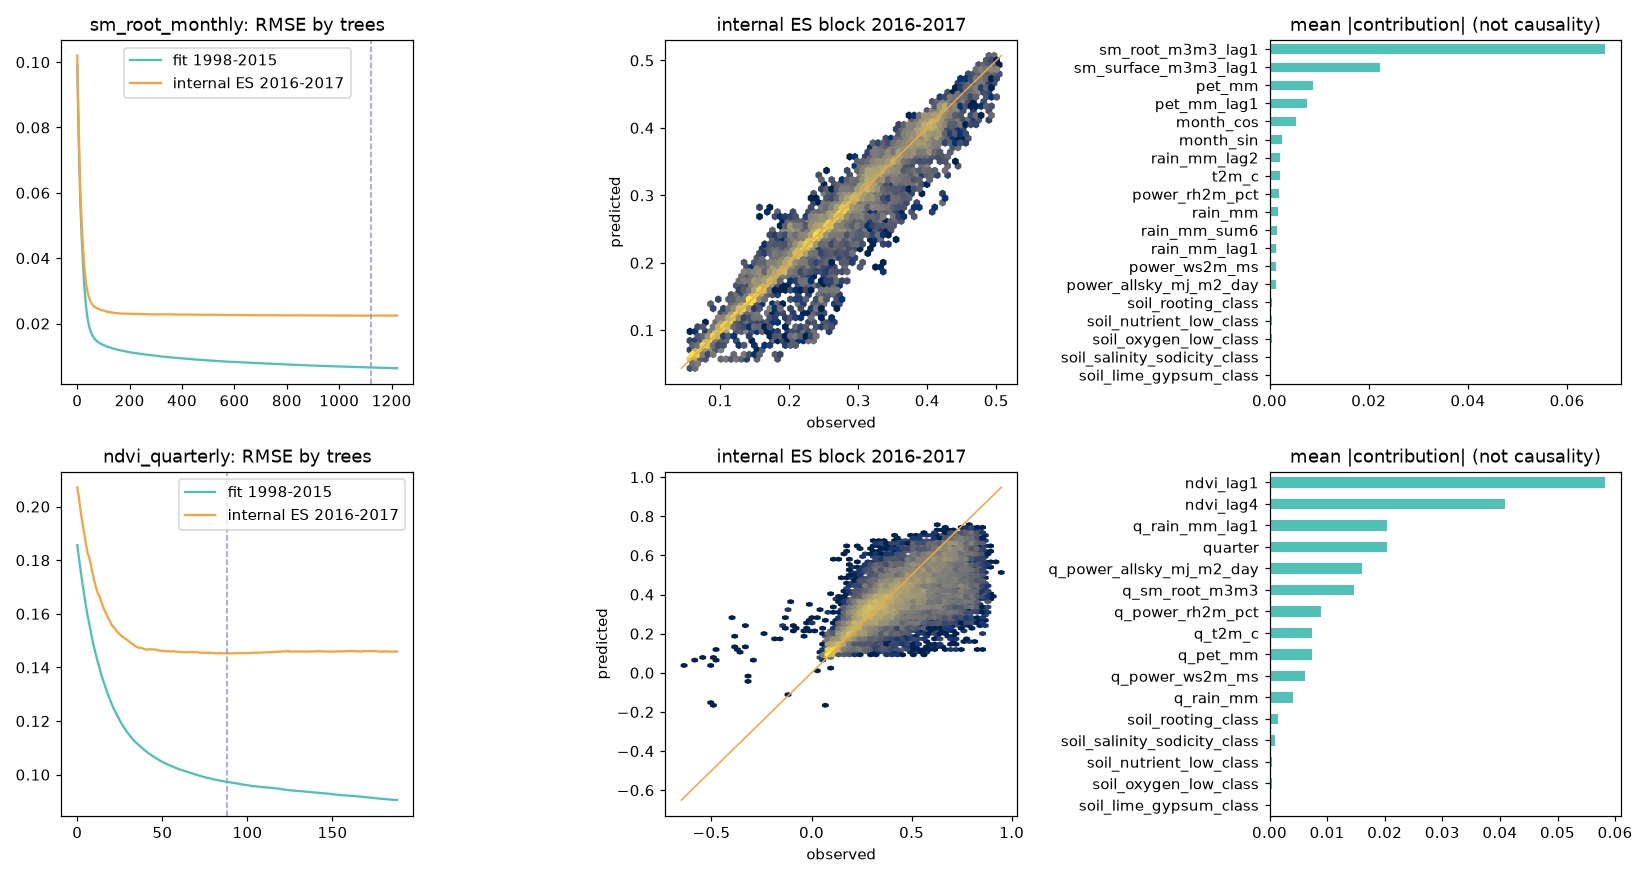
\includegraphics[width=\textwidth]{figures/phase1_diagnostics.png}
\caption{Phase 1 diagnostics: learning curves with early stopping, predicted against observed values on 2016--2017,
and mean absolute TreeSHAP contributions of the features.}
\label{fig:p1}
\end{figure}

\subsection{Validation (2018--2022)}
The frozen models were evaluated on five new years with new NASA POWER files (Table~\ref{tab:val}). Both pass every
criterion (Table~\ref{tab:valcrit}). The NDVI model passes by a small margin: the lower bound of its skill sits exactly at
the threshold, and in Ferre\~nafe province it is barely better than climatology.

\begin{table}[H]
\centering\small
\caption{Validation 2018--2022 (95\,\% block bootstrap CI).}
\label{tab:val}
\begin{tabular}{lcccc}
\toprule
& MAE & RMSE & $R^2$ & Bias \\
\midrule
\multicolumn{5}{l}{\textit{Soil water, \sm{} (187,560 rows)}} \\
XGBoost & 0.0073 \ci{0.0061}{0.0084} & 0.0125 \ci{0.0110}{0.0139} & 0.986 \ci{0.981}{0.990} & $-0.0004$ \\
Persistence & 0.0139 & 0.0260 & 0.940 & 0.0002 \\
Climatology & 0.0212 & 0.0317 & 0.911 & 0.0074 \\
\midrule
\multicolumn{5}{l}{\textit{NDVI (50,477 rows)}} \\
XGBoost & 0.075 \ci{0.070}{0.079} & 0.103 \ci{0.097}{0.109} & 0.66 \ci{0.60}{0.72} & 0.002 \\
Climatology & 0.089 & 0.126 & 0.50 & $-0.031$ \\
Persistence & 0.107 & 0.156 & 0.22 & 0.005 \\
\bottomrule
\end{tabular}
\end{table}

\begin{table}[H]
\centering\small
\caption{Acceptance criteria on Validation.}
\label{tab:valcrit}
\begin{tabular}{llll}
\toprule
& Rule & Soil water & NDVI \\
\midrule
A & skill vs best baseline & 0.52 \ci{0.48}{0.55} vs persistence & 0.18 \ci{0.10}{0.25} vs climatology \\
B & lower CI $>0$ & 0.48 & 0.10 \\
C & RMSE & 0.0125 & 0.103 (report) \\
D & $|$bias$|$ & 0.0004 & 0.002 \\
E & worst year / province & 0.45 / 0.28 & 0.06 / 0.01 \\
F & 90\,\% coverage 2021--2022 & 0.872 (edge) & 0.880 \\
G & rows outside p01--p99 & 15\,\% & 16\,\% \\
\midrule
& \textbf{Verdict} & \textbf{accepted} & \textbf{accepted} \\
\bottomrule
\end{tabular}
\end{table}

The final 90\,\% half-widths, calibrated on all of 2018--2022, were $\pm0.013$\,\sm{} (dry season) and $\pm0.030$\,\sm{}
(wet season) for soil water, and $\pm0.12$ to $\pm0.20$ by quarter for NDVI.

\begin{figure}[H]
\centering
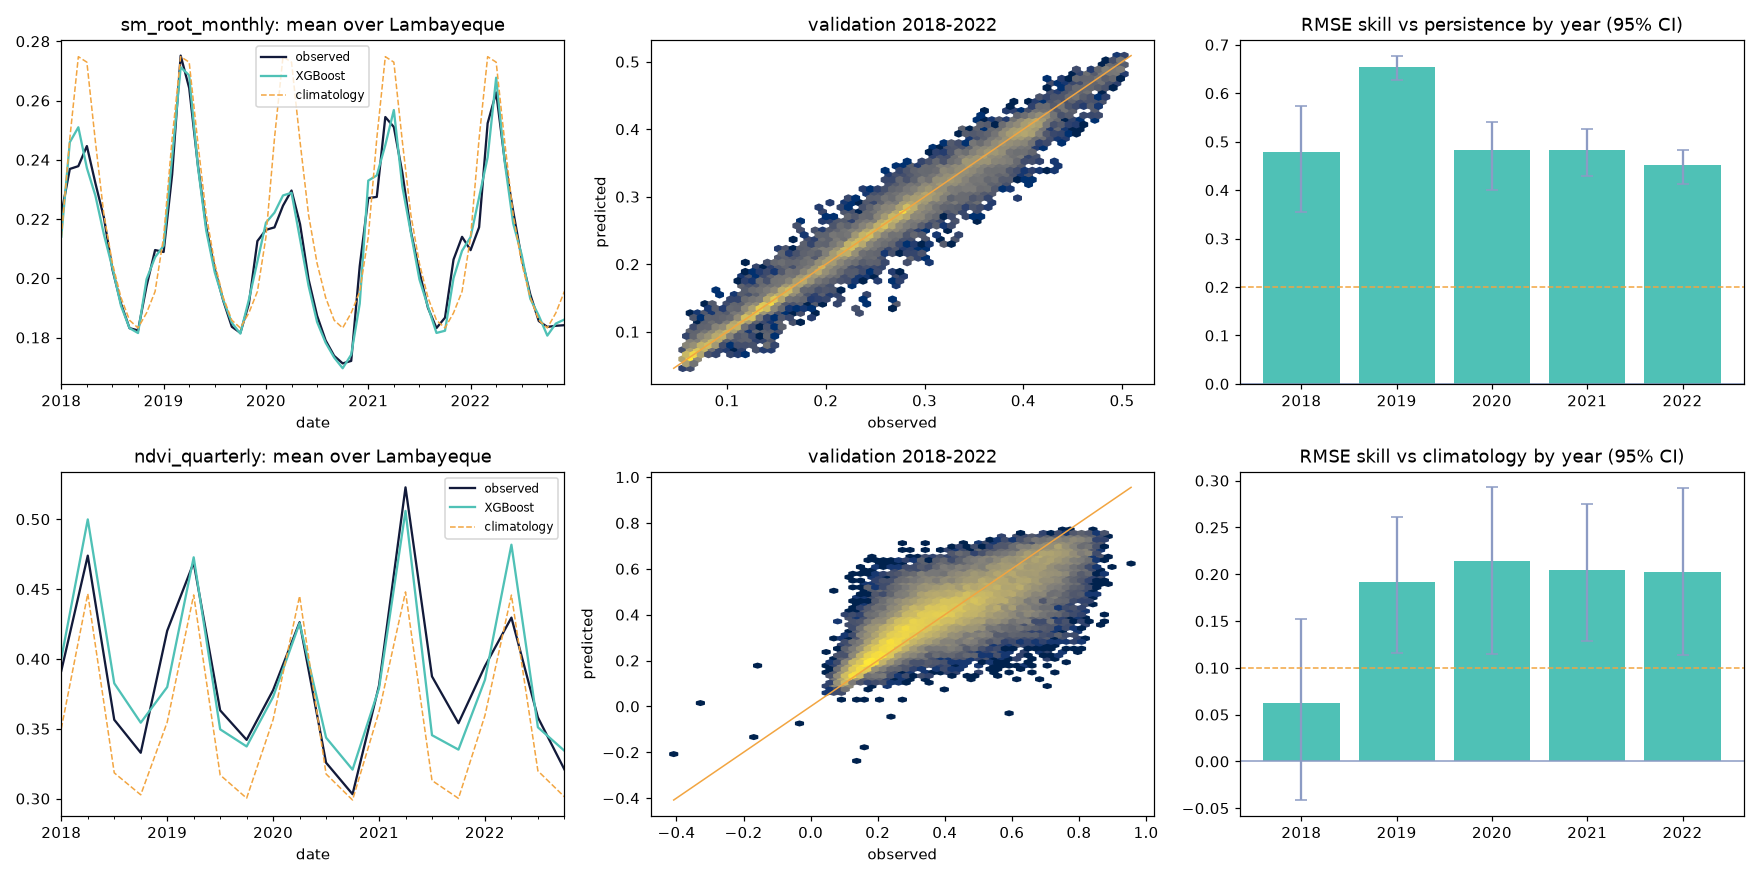
\includegraphics[width=\textwidth]{figures/phase2_validation.png}
\caption{Validation 2018--2022: grid-mean observed values, model predictions and climatology.}
\label{fig:p2}
\end{figure}

\subsection{Testing (2023--2025)}
The test was run once, with the models unchanged (their SHA-256 hashes were checked against Validation). The period
contains the wettest month of the record, March 2023 (119\,mm on average over the grid).

\begin{table}[H]
\centering\small
\caption{Testing 2023--2025 (95\,\% CI).}
\label{tab:test}
\begin{tabular}{lcc}
\toprule
& Soil water (112,536 rows) & NDVI (30,056 rows) \\
\midrule
MAE & 0.0113 \ci{0.0103}{0.0123} & 0.094 \ci{0.090}{0.097} \\
RMSE & 0.0198 \ci{0.0185}{0.0211} & 0.126 \ci{0.121}{0.131} \\
$R^2$ & 0.962 \ci{0.954}{0.968} & 0.53 \ci{0.48}{0.57} \\
Bias & $-0.0030$ \ci{-0.0036}{-0.0024} & $-0.026$ \ci{-0.032}{-0.020} \\
MAPE & 5.1\,\% & --- \\
Skill vs baseline & 0.46 \ci{0.44}{0.49} (persistence) & 0.21 \ci{0.14}{0.29} (climatology) \\
Criteria A--E & pass & pass \\
90\,\% coverage (criterion F) & \textbf{82\,\%} \ci{80}{84}: fails & \textbf{84--85\,\%}: fails \\
\bottomrule
\end{tabular}
\end{table}

Both models keep beating the simple rules, including in the El Ni\~no year. Their intervals, however, are too narrow:
the ``90\,\%'' band covered 82\,\% of soil water values (77\,\% in the wet season and in 2023) and 84\,\% of NDVI values. The
worst periods are March 2023 for soil water (RMSE 0.053, bias $-0.037$: the model fills the soil less than the El Ni\~no
did) and the second quarter of 2023 for NDVI (bias $-0.15$: the greening after the rains is missed). Between 18 and
21\,\% of test rows had at least one input outside the training p01--p99 range.

\begin{figure}[H]
\centering
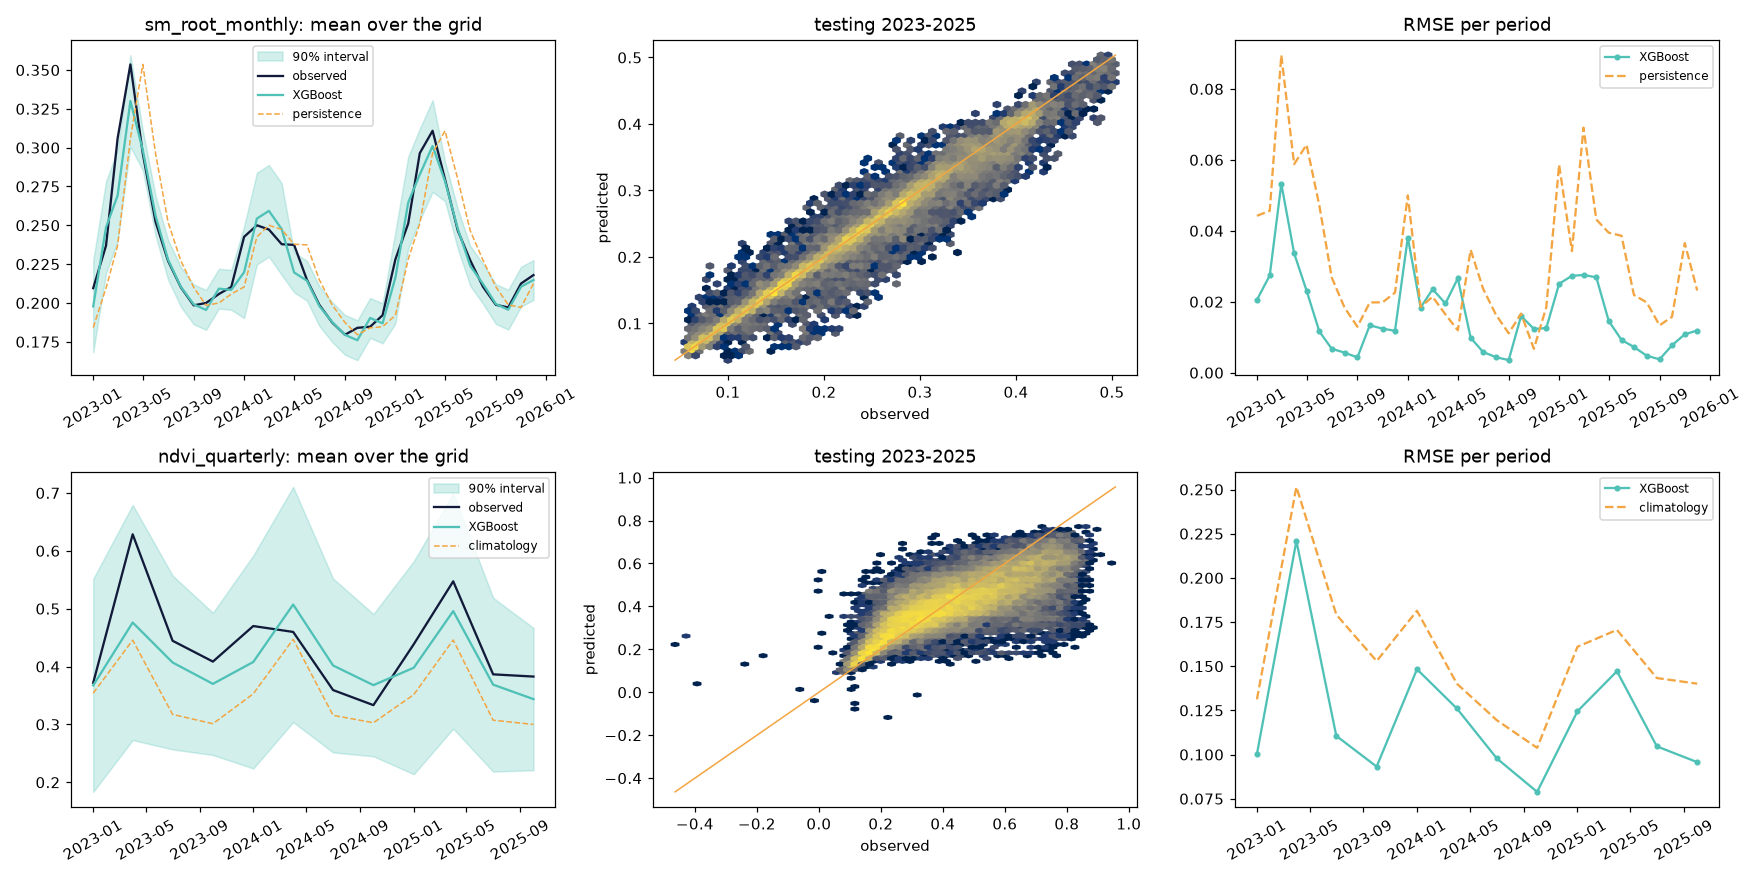
\includegraphics[width=\textwidth]{figures/phase3_testing.png}
\caption{Testing 2023--2025: grid-mean observed values, predictions and the 90\,\% interval calibrated in Validation.}
\label{fig:p3}
\end{figure}

\begin{table}[H]
\centering\small
\caption{The same (v1) models across the three phases.}
\label{tab:phases}
\begin{tabular}{lccc}
\toprule
& Training (internal 2016--17) & Validation 2018--22 & Testing 2023--25 \\
\midrule
Soil water RMSE ($R^2$) & 0.022 (0.955) & 0.013 (0.986) & 0.020 (0.962) \\
Soil water skill vs persistence & 0.48 & 0.52 \ci{0.48}{0.55} & 0.46 \ci{0.44}{0.49} \\
NDVI RMSE ($R^2$) & 0.145 (0.49) & 0.103 (0.66) & 0.126 (0.53) \\
NDVI skill vs climatology & 0.08 & 0.18 \ci{0.10}{0.25} & 0.21 \ci{0.14}{0.29} \\
\bottomrule
\end{tabular}
\end{table}

% ==================================================================================================================
\section{Evolution of the research after the test}\label{sec:evolution}
The test answered ``is it accurate?'' but opened three questions from the team and the event mentors: why did the
intervals fail, can El Ni\~no be taught to the model, and can the models look ahead? Each experiment below left the
tested models untouched and had its rules committed before it ran. Because 2023--2025 had already been used by the test,
results on those years are a \emph{second look}, not an independent test.

\subsection{Why the intervals failed}
The soil water model fits its own years 2--3 times better than new years (in-sample RMSE 0.007 against 0.013 and 0.020),
the usual optimism of boosted trees, but its skill over persistence is the same in every phase. More regularisation would
reduce the in-sample error, not the error on new years. The diagnosis pointed elsewhere:
\begin{enumerate}
\item \textbf{Error grows with rain, the interval does not.} In months of 30--60\,mm the soil water error is 2--3.5 times that
of dry months, and the season-wide interval covered only 71\,\% of them.
\item \textbf{Drift.} In 2023--2025 the error doubled even in months without rain (0.004 to 0.009\,\sm): conditions moved
away from the training years.
\item \textbf{El Ni\~no is not among the inputs.}
\end{enumerate}

\subsection{Adaptive intervals: CQR and monthly recalibration}
Two remedies that need no new data were combined. Conformalized quantile regression \citep{romano2019} trains XGBoost
quantile models (5\,\% and 95\,\%) on 1998--2017 and corrects them on Validation, so the band widens in months that were
hard in the past. Adaptive conformal inference \citep{gibbs2021} then recalibrates the band each month from the errors
of the last three years, raising its level after a month that missed too often; its step $\gamma=0.2$ was chosen on
Validation. Intervals are compared by coverage and by the interval score \citep{gneiting2007}, which rewards narrow
bands and penalises misses.

\begin{table}[H]
\centering\small
\caption{90\,\% intervals on 2023--2025 (coverage [95\,\% CI], mean width, interval score; lower score is better).}
\label{tab:cqr}
\begin{tabular}{lccc}
\toprule
Interval & Soil water & NDVI & Score (soil, NDVI) \\
\midrule
v1 (tested, one width per season) & 82\,\% \ci{79}{84}, 0.037 & 84\,\% \ci{83}{85}, 0.33 & 0.102, 0.56 \\
CQR & 82\,\% \ci{81}{84}, 0.039 & 86\,\% \ci{84}{87}, 0.35 & 0.082, 0.50 \\
v1 + monthly recalibration & 90\,\% \ci{89}{92}, 0.063 & 87\,\% \ci{86}{88}, 0.36 & 0.097, 0.56 \\
\textbf{CQR + monthly recalibration} & \textbf{90\,\%} \ci{89}{91}, 0.051 & \textbf{89\,\%} \ci{88}{90}, 0.39 & \textbf{0.081, 0.49} \\
\bottomrule
\end{tabular}
\end{table}

CQR with monthly recalibration reaches the promised 90\,\% in both models and has the best interval score; the price is a
wider band ($\pm0.026$ instead of $\pm0.018$\,\sm). The wet-season coverage of soil water rose from 77 to 89\,\%. Single
extreme months remain: in March 2023 and May 2024 only about half of the cells fell inside the band
(Figure~\ref{fig:aci}). Recalibration fixes the average, not the month of the shock.

\begin{figure}[H]
\centering
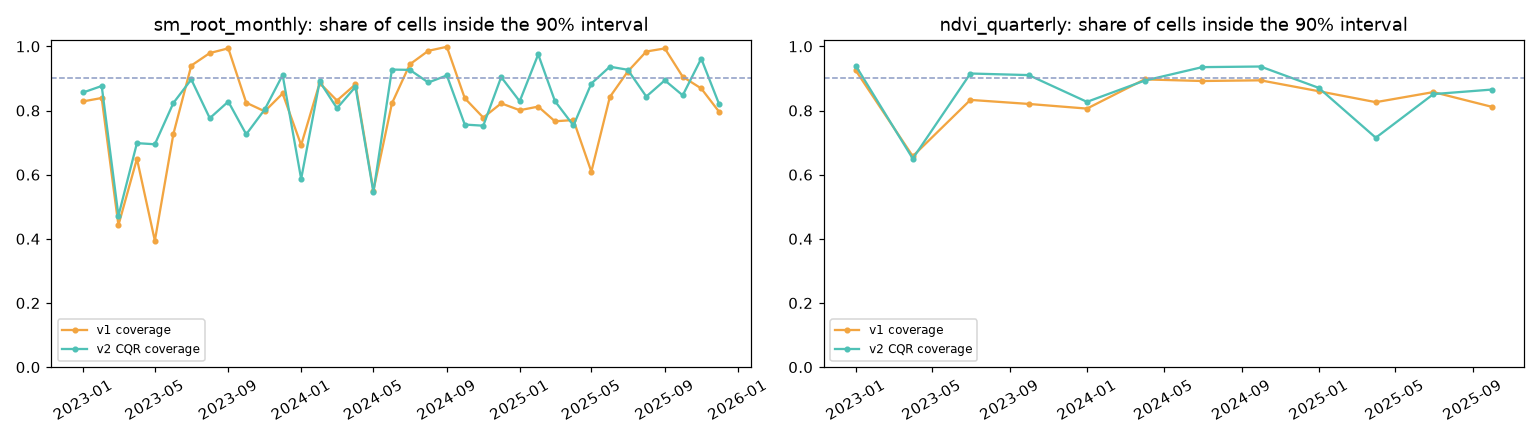
\includegraphics[width=\textwidth]{figures/v2_coverage.png}\\[4pt]
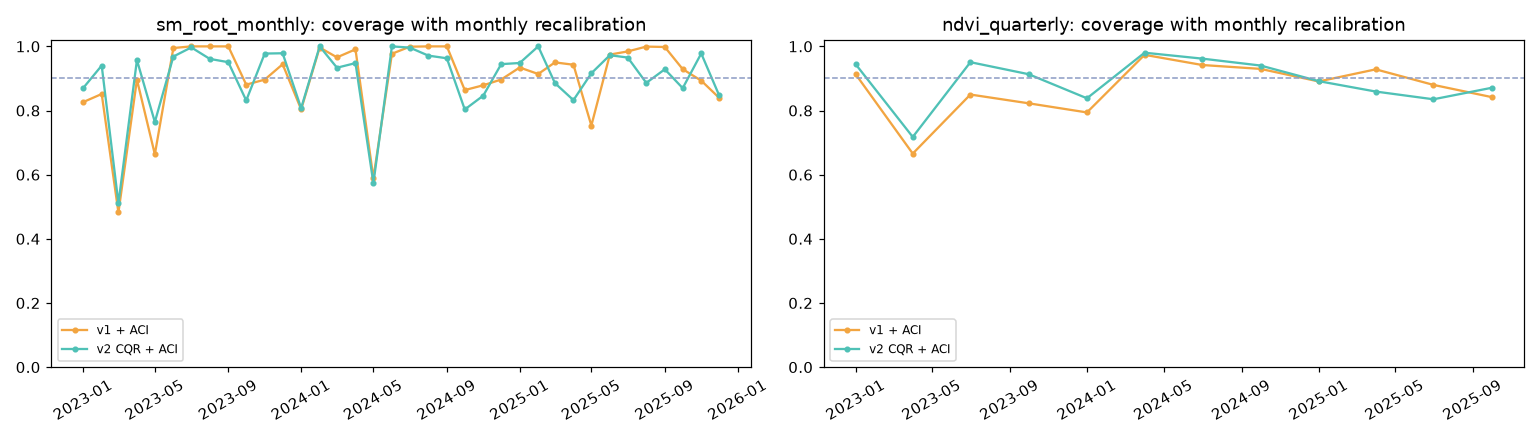
\includegraphics[width=\textwidth]{figures/v2_aci_coverage.png}
\caption{Share of cells inside the 90\,\% band per period in 2023--2025. Top: tested intervals against CQR. Bottom: both with
monthly recalibration (ACI). The dashed line is the nominal 90\,\%.}
\label{fig:aci}
\end{figure}

\subsection{Teaching El Ni\~no to the model}\label{sec:nino}
We then received two datasets. The NOAA PSL Ni\~no~1+2 anomaly (monthly, 1870--September 2026) was complete for
1998--2025; its header declares $-99.99$ as missing but the last months use $-9999$, both treated as missing. The second
file, requested from the Copernicus data store as ERA5 precipitation, turned out to be the \emph{hourly} ERA5 product at
0.25$^\circ$ for 1998--2004 with a single hour per day (00\,UTC): its ``rain'' is one hour out of 24, and scaled to a month it
gave 955\,mm a year against 220\,mm from CHIRPS. It was not used, and we documented the right request (ERA5-Land monthly
aggregates), which later led to the v3 model (Section~\ref{sec:v3}).

New features were added and nothing else changed: the Ni\~no~1+2 anomaly of the month, of the previous month and its
three-month mean (soil water), and the quarter mean and previous quarter (NDVI). The decision rule, committed before
training, compared v2 with v1 on Validation by the skill $1-\mathrm{RMSE}_{v2}/\mathrm{RMSE}_{v1}$.

\begin{table}[H]
\centering\small
\caption{v2 models with the Ni\~no~1+2 index. Validation decides; 2023--2025 is a second look.}
\label{tab:nino}
\begin{tabular}{lcc}
\toprule
& Soil water & NDVI \\
\midrule
Skill of v2 over v1, Validation 2018--2022 & $-0.009$ \ci{-0.031}{0.010} & $-0.013$ \ci{-0.021}{-0.005} \\
Criteria A--F on Validation & all pass & E fails (one province $-0.016$) \\
\textbf{Verdict} & \textbf{no difference: decided on 2026} & \textbf{rejected} \\
\midrule
RMSE 2023--2025, v1 $\to$ v2 & 0.0198 $\to$ 0.0185 & 0.126 $\to$ 0.121 \\
Peak of El Ni\~no, v1 $\to$ v2 & March 2023: 0.053 $\to$ 0.039 & Q2 2023: 0.221 $\to$ 0.182 \\
Calm years (2024, 2025) & unchanged & slightly worse in 2025 \\
\bottomrule
\end{tabular}
\end{table}

The index cuts the error of the El Ni\~no peak by a fifth to a quarter but adds nothing, or some noise, in the calm
validation years (Figure~\ref{fig:nino}), where no strong event occurred. With only a few events in 1998--2017, the trees
can use the index partly as a label for those years. By the rules, v1 remained the standard model; the soil water v2 waits
for 2026, whose Ni\~no~1+2 anomaly reached $+3.85\,^\circ$C in September 2026, stronger than 2023.

\begin{figure}[H]
\centering
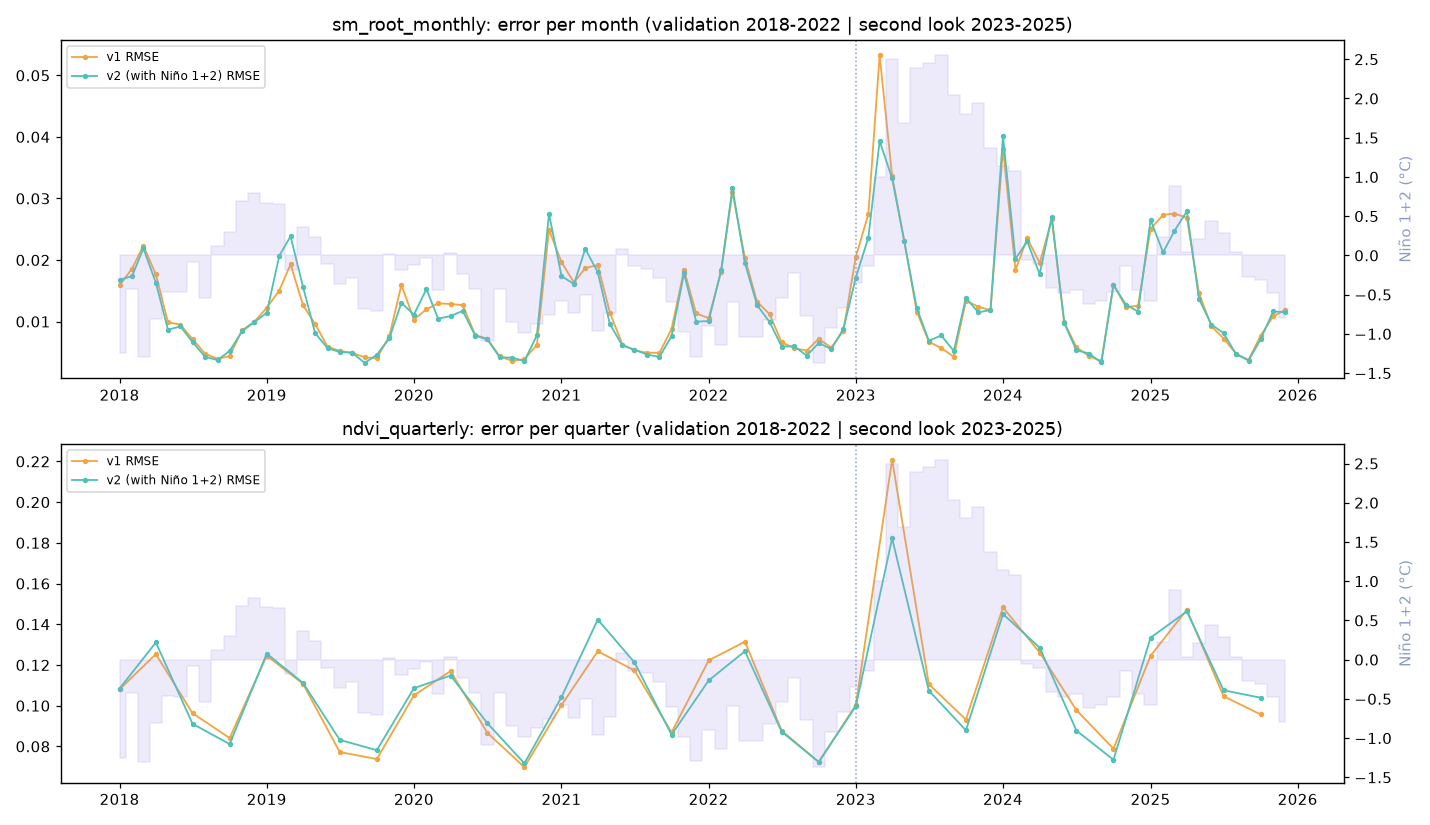
\includegraphics[width=\textwidth]{figures/v2_nino_error_timeline.png}
\caption{Error per month (soil water) and per quarter (NDVI) of v1 and v2, with the Ni\~no~1+2 anomaly in the background.
The dotted line separates Validation from the second look at 2023--2025.}
\label{fig:nino}
\end{figure}

\subsection{Projections and what-if scenarios}\label{sec:proj}
The tested models describe a month from \emph{that month's} weather; looking ahead needs the weather of months that have
not happened. We used an analog ensemble, known in hydrology as Ensemble Streamflow Prediction \citep{day1985}: from the
observed state of each cell, the coming months are simulated once with the weather of each past year, feeding each
predicted soil water value into the next month; the NDVI model runs on the simulated quarters. The band is the 5--95\,\%
range of the members widened by a per-lead correction calibrated on Validation hindcasts (a conformalized band). A
consistency check confirmed that with the real weather the first month equals the tested model's own prediction exactly.

Hindcasts started every month from December 2017 to November 2022 (leads 1--12 months for soil water, 1--4 quarters for
NDVI), with analog years 1998--2017 and no analog month after December 2017. The \emph{useful lead} was defined in advance as
the longest lead whose skill against the better simple rule has a lower 95\,\% bound above zero at every shorter lead.

\begin{table}[H]
\centering\small
\caption{Projection skill by lead with the v1 models (95\,\% CI). Validation hindcasts decide; 2023--2025 is reported only.}
\label{tab:lead}
\begin{tabular}{lcc|lcc}
\toprule
Soil water lead & 2018--2022 & 2023--25 & NDVI lead & 2018--2022 & 2023--25 \\
\midrule
1 month & 0.39 \ci{0.34}{0.43} & 0.35 & 1 quarter & 0.17 \ci{0.09}{0.25} & 0.19 \\
2 & 0.18 \ci{0.14}{0.23} & 0.09 & 2 & 0.11 \ci{0.03}{0.19} & 0.12 \\
3 & 0.08 \ci{0.05}{0.13} & 0.01 & 3 & 0.11 \ci{0.03}{0.18} & 0.13 \\
6 & 0.04 \ci{0.005}{0.09} & $-0.09$ & 4 & 0.10 \ci{0.07}{0.13} & 0.12 \\
12 & 0.01 \ci{-0.03}{0.06} & $-0.13$ & & & \\
\bottomrule
\end{tabular}
\end{table}

The useful lead is 6 months for soil water and 4 quarters for NDVI, with most of the gain in the first 2--3 months. In the
El Ni\~no period 2023--2025 soil water projections beat climatology only for 2 months. The 90\,\% bands covered 80\,\%
\ci{79}{82} (soil water) and 84\,\% \ci{83}{86} (NDVI) of the 2023--2025 values, again too narrow in an extreme period.

\paragraph{First scenario sanity checks.} Two checks were pre-registered: two months without rain must not raise soil water, and
doubling the rain must not lower it, in more than 1\,\% of the cells. Both \textbf{failed} (25\,\% and 38\,\% of the cells on
average). The drought scenario, which removes the rain and sets the surface soil to its driest observed value, does dry
the soil clearly ($-0.04$\,\sm{} for January starts), and the cells that ``rise'' show small tree-step changes. Rain alone,
however, barely moved the v1 model: doubling it changed soil water by at most $+0.003$\,\sm{} on average, less than the model
error. The reason is in the model itself: last month's root-zone soil water carries 68\,\% of the gain and the surface
soil 24\,\%, while the four rain inputs add up to 2.4\,\%. Following the rule, rain-only scenarios were not offered to
users at that point; Sections~\ref{sec:checks} and~\ref{sec:v3} show how this was later solved.

\begin{figure}[H]
\centering
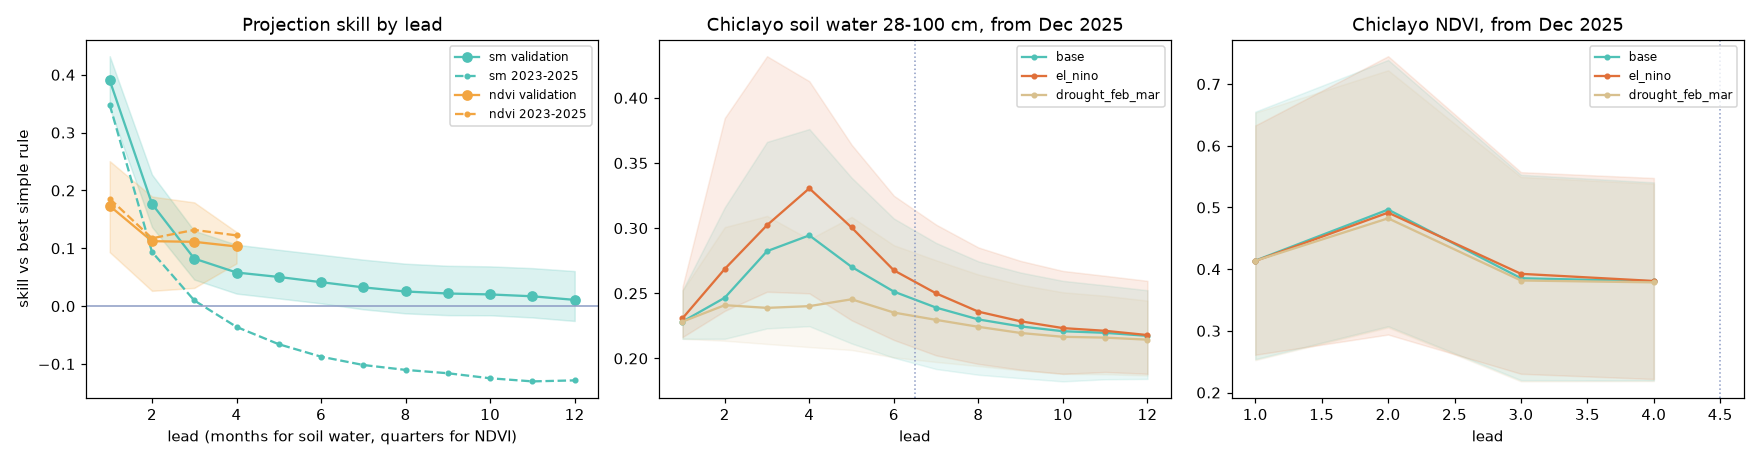
\includegraphics[width=\textwidth]{figures/projections_overview.png}
\caption{Left: projection skill by lead (v1), Validation hindcasts (with 95\,\% CI) and 2023--2025. Centre and right: projections
from December 2025 for Chiclayo province (mean of cells) in a normal year, in El Ni\~no years and with two months without
rain; the dotted line marks the useful lead.}
\label{fig:proj}
\end{figure}

% ==================================================================================================================
\section{Checks before serving new features}\label{sec:checks}
A teammate proposed a full API with predictions by cell, typed simulations (drought, El Ni\~no, temperature, rain,
recovery), territorial analysis, alerts and explanations. Before writing any endpoint we wrote, for each new feature, a
check that decides whether it may be served as validated or only with the label \emph{experimental}
(Table~\ref{tab:checks}). The first scenario checks had counted any move above $10^{-4}$\,\sm{} as ``wrong direction'';
those results stand. The new checks, written knowing that result, ask a different question: \emph{does a scenario move
soil water in the wrong direction by more than the model's own error} (validation RMSE 0.0125\,\sm)? All scenario checks
start at the end of every month from December 2017 to December 2021 (49 starts), on the 1,950 Lambayeque cells.

\begin{table}[H]
\centering\small
\caption{Checks written before the API expansion, run with the tested v1 models (notebook 07).}
\label{tab:checks}
\begin{tabularx}{\textwidth}{l>{\raggedright\arraybackslash}p{3.3cm}>{\raggedright\arraybackslash}Xl}
\toprule
& Feature & Rule (shortened) and result & Verdict \\
\midrule
S1 & Temperature what-if & $+2\,^\circ$C must not raise soil water by more than the error in $>1$\,\% of cells. It did in 9.7\,\% (mean $+0.0024$, the wrong way) & fail \\
S2 & Droughts of 1--6 months & Mean change negative, longer not wetter, $\le1$\,\% of cells rising. Lengths 1--4 pass; 5 and 6 months reach 1.4 and 2.5\,\% & fail \\
S3 & Rain-only what-if & Few wrong-way moves (0.15 / 0.46\,\%), but mean effect $\pm0.0006$\,\sm, a twentieth of the error (needs $\ge0.003$) & fail \\
S4 & Recovery after 3 dry months & Difference at lead 12 smaller than at lead 3 in $\ge90$\,\% of cells: 83\,\% & fail \\
S5 & Drought risk (share of analog members below the cell's 20th percentile) & Calibration within 0.10 in every bin: predicted 0.95 $\to$ observed 0.65. Brier skill 0.18 against a constant 0.20 & fail \\
S6 & Alerts (value below the lead-1 band) & Share of cells flagged in 2018--2022 between 2.5 and 10\,\%: 4.7\,\% soil water, 3.7\,\% NDVI & \textbf{pass} \\
S7 & NDVI greener than expected (possible irrigation) & No independent irrigated-area data: 591 cells above the model in $\ge3$ of 8 quarters, unverified & not testable \\
S8 & The 1,176 cells outside Lambayeque & Criteria A--E on 2018--2022: soil water skill 0.54 \ci{0.50}{0.58}, NDVI 0.12 \ci{0.05}{0.18} & \textbf{pass} \\
S9 & Adaptive ranges in the API & Needs complete 2026 data & deferred \\
S10 & Per-cell confidence & Spearman correlation between a place's validation and test error: 0.65 over 226 ERA5-Land pixel groups & \textbf{pass} \\
\bottomrule
\end{tabularx}
\end{table}

Three checks passed and five failed. The API serves alerts, per-cell confidence and the outer cells as validated (level
\texttt{warning}, never \texttt{ok}, because they are still model outputs), and everything else as
\texttt{experimental} with the reason. The lesson was concrete: the v1 model answers a change of one input mostly through
last month's soil water, so it moves little and sometimes the wrong way. Simulations need a model that \emph{reacts} to
the weather it is given.

% ==================================================================================================================
\section{A third soil water model with ERA5-Land's own rain (v3)}\label{sec:v3}

\subsection{The new data}
Following our request, the team exported from Google Earth Engine the ERA5-Land monthly aggregates
(\texttt{ECMWF/ERA5\_LAND/MONTHLY\_AGGR}) on a 2\,km covering grid: 9,016 cells $\times$ 346 months (January 1998 to October
2026), 3.1 million rows, no duplicates. Our 3,149 cells are all present with the same identifiers; 22 coastal cells have no
value (the same land--sea mask). Soil water layer 2 (7--28\,cm) is coherent ($r=0.94$ with layer 3, between layers 1 and 3 in
92\,\% of cell-months).

The precipitation follows CHIRPS over time ($r=0.81$ for the monthly grid mean, 0.54 cell by cell) but is \textbf{3--6 times
larger}: 923 against 221\,mm in 2000, 3,069 against 337\,mm in 1998, 650 against 153\,mm in 2024. It is not a unit error:
the hourly file had given the same order. Reanalysis rain is known to be too wet over this coast and the Andes. We
nevertheless used it, \emph{as a model input only}, because it is the rain that drives the ERA5-Land soil water we predict;
it is never shown to users as ``the rain''.

\subsection{Rules written before training}
v3 changes only the soil water model; the NDVI model stays the tested v1. Features: the 19 v1 features plus
\texttt{era5\_rain\_mm}, its two lags and its six-month sum, built like the CHIRPS ones inside each cell. Layer 2 was
\emph{not} used: a same-month value sits next to the target, and a lagged one would be another state the projections
cannot predict. We added \textbf{monotone constraints} \citep{chen2016}: $+1$ for the eight rain features (more rain never
lowers the prediction) and $-1$ for potential evaporation and temperature (more evaporative demand or heat never raises
it). Everything else as v1: target, hyperparameters, seed, fit 1998--2015, early stopping on 2016--2017, refit on 1998--2017.

The decision rules were: \textbf{R1}, criteria A--F with the same thresholds; \textbf{R2}, v3 not clearly worse than v1
(the upper 95\,\% bound of the skill of v3 over v1 is $\ge0$); \textbf{R3}, rerun checks S1--S4, each pass removing the
\texttt{experimental} label of that scenario when v3 runs it; \textbf{R4}, projection hindcasts for v3's own useful lead and
range corrections; \textbf{R5}, 2023--2025 reported only. If R1 or R2 failed, v3 would not be used.

\subsection{Results}

\begin{table}[H]
\centering\small
\caption{v1 against v3 (soil water). Validation decides; 2023--2025 is a second look.}
\label{tab:v3}
\begin{tabular}{lcc}
\toprule
& v1 & \textbf{v3} \\
\midrule
Trees & 1,122 & 1,877 \\
Validation 2018--2022 RMSE (\sm) & 0.0125 \ci{0.0110}{0.0139} & \textbf{0.0099} \ci{0.0087}{0.0110} \\
Skill vs persistence (A, B) & 0.52 \ci{0.48}{0.55} & \textbf{0.62} \ci{0.59}{0.64} \\
Skill of v3 over v1 (R2) & --- & $\mathbf{+0.21}$ \ci{0.17}{0.25} \\
Criteria A--F (R1) & pass (F at the edge, 0.872) & pass (bias $-0.0013$, worst year 0.56, worst province 0.44, F 0.884) \\
2023--2025 RMSE & 0.0198 & \textbf{0.0142} (skill over v1 $+0.28$ \ci{0.24}{0.32}) \\
March 2023 RMSE / bias & 0.053 / $-0.037$ & \textbf{0.024} / $-0.007$ \\
90\,\% one-step interval, wet / dry season & $\pm0.030$ / $\pm0.013$ & $\pm$\textbf{0.020} / $\pm0.013$ \\
Its coverage in 2023--2025 & 82\,\% & 82\,\% \\
Share of gain: last month's soil / surface / rain & 68 / 24 / 2.4\,\% & 65 / 22 / \textbf{8.3}\,\% \\
\bottomrule
\end{tabular}
\end{table}

R1 and R2 pass, and not just as ``not worse'': v3 cuts the validation error by a fifth with a confidence interval far from
zero. The gain is largest where v1 failed: the March 2023 coastal El Ni\~no error is halved and its bias almost vanishes.
The rain inputs now carry 8.3\,\% of the gain (8.0\,\% from ERA5-Land rain, 0.3\,\% from CHIRPS), so the model learned
to use the rain that drives its target.

\begin{table}[H]
\centering\small
\caption{Scenario checks (Section~\ref{sec:checks}) rerun with v3, same rules and starts.}
\label{tab:v3checks}
\begin{tabularx}{\textwidth}{l>{\raggedright\arraybackslash}p{4.2cm}X}
\toprule
Check & v1 & v3 \\
\midrule
S1 temperature $\pm2\,^\circ$C & fail (9.7\,\% wrong way) & \textbf{pass}: 0\,\% wrong way; $+2\,^\circ$C lowers soil water by 0.003 on average, $-2\,^\circ$C raises it by 0.003 \\
S2 droughts of 1--6 months & fail (5--6 months) & \textbf{pass}: $-0.007$, $-0.019$, $-0.030$, $-0.039$, $-0.046$, $-0.052$\,\sm{} at the end of the drought; $\le0.01$\,\% of cells rise \\
S3 rain $\times0.5$ / $\times2$ & fail (effect $\pm0.0006$) & \textbf{pass}: $-0.012$ / $+0.019$\,\sm, no cell the wrong way \\
S4 recovery after 3 dry months & fail (83\,\%) & \textbf{fail} (76\,\%): the effect fades by month 12 on average ($-0.030 \to -0.007$), but not in $\ge90$\,\% of cells \\
\bottomrule
\end{tabularx}
\end{table}

\paragraph{Projections and intervals with v3.} The hindcasts of R4 give v3 the same useful lead as v1 (6 months; skill
0.43 at lead 1 against persistence, 0.17 at lead 2 against climatology) and a 90\,\% band that covered 81\,\% of the
2023--2025 values (v1: 80\,\%). In 2023--2025 the projection beats climatology only for the first 2 months, as v1 did:
v3 describes a month better, but it cannot know next year's weather any better than the analog years do. Two more
measurements were needed to put v3 in the whole tool, both with the same code and rules as v1: the NDVI projections fed
with v3's soil water stay useful for 4 quarters (skill 0.17, 0.11, 0.11, 0.10, every lower bound above zero) and their
band covered 84\,\% in 2023--2025, as with v1; the one-step interval, computed with the code that reproduces v1's stored
widths exactly, is $\pm0.020$\,\sm{} in the wet season instead of $\pm0.030$, with the same real coverage (82\,\%).
Figure~\ref{fig:v3} summarises the comparison.

\begin{figure}[H]
\centering
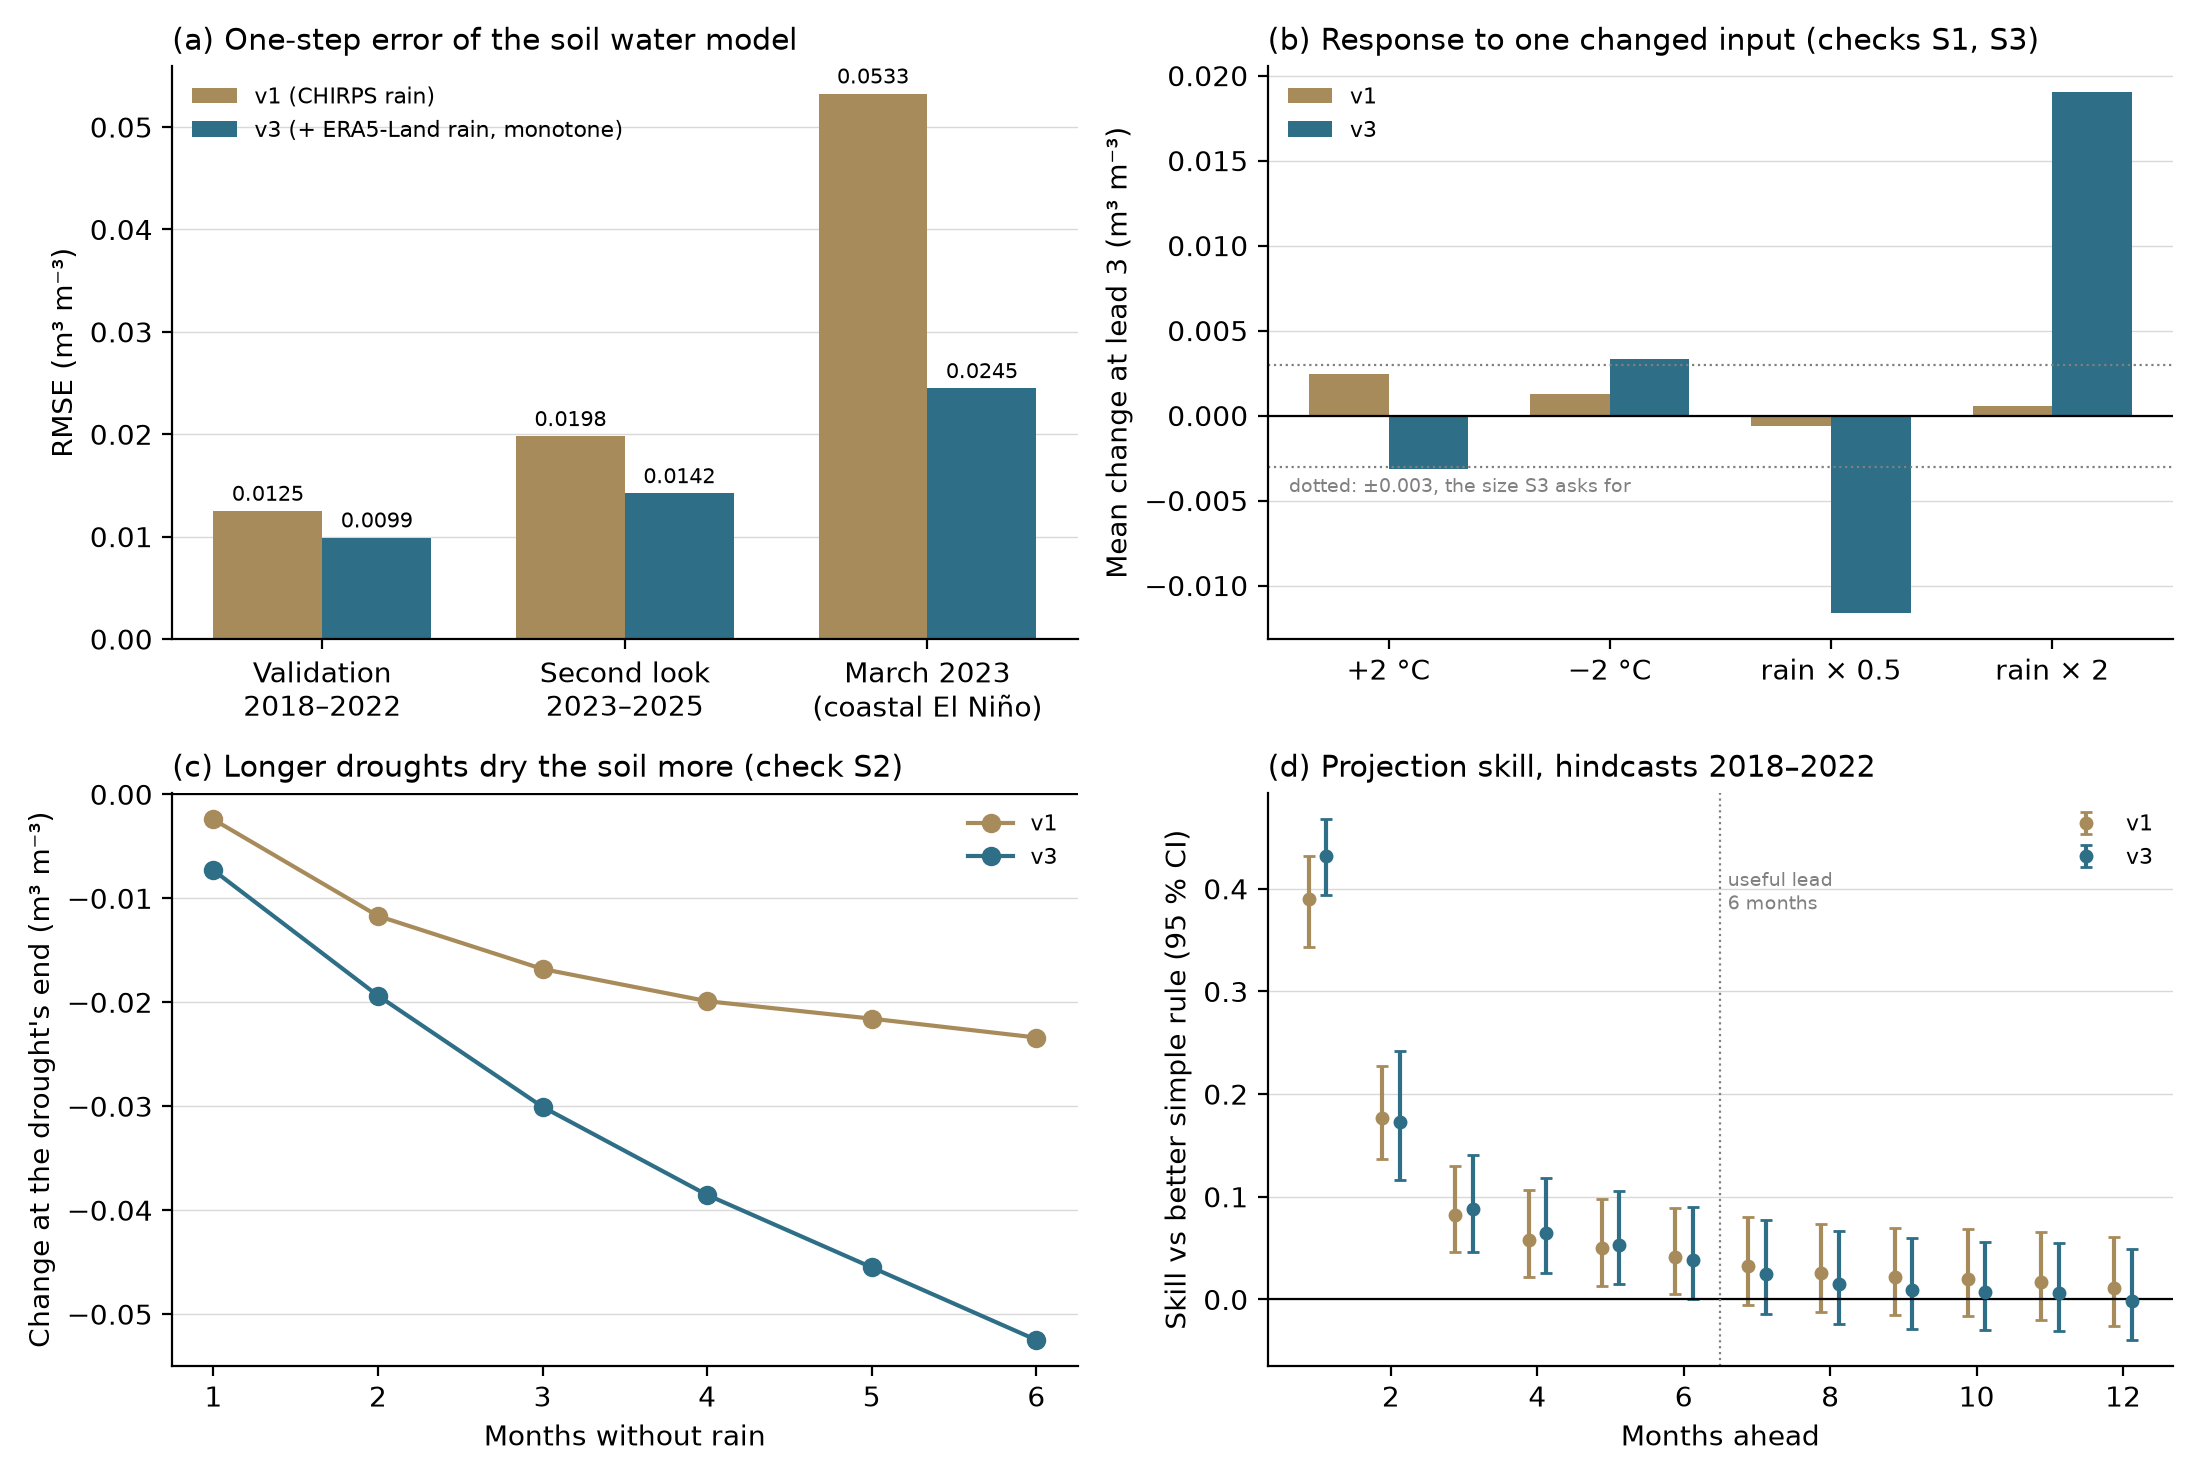
\includegraphics[width=\textwidth]{figures/v3_overview.png}
\caption{v1 against v3. (a) One-step error by period. (b) Mean change of soil water at lead 3 when one input changes;
the dotted lines are the size check S3 asks for. (c) Mean change at the end of droughts of 1--6 months. (d) Projection skill
by lead in the Validation hindcasts (95\,\% CI); both models are useful for 6 months.}
\label{fig:v3}
\end{figure}

\paragraph{What passing means.} The checks S1--S3 ask whether the model moves in the physically expected direction and by
a visible amount; they cannot tell whether $-0.030$\,\sm{} after three dry months is the \emph{right} amount, because no
year offers the same months with and without rain. The scenarios therefore remain the model's answer to a made-up
situation, not a forecast. With these results, and following the rules, the team decided on November 15, 2026 to use v3
for every soil water number of the tool (Section~\ref{sec:tool}); the alerts stay on v1 because check S6 was validated with it.

% ==================================================================================================================
\section{From models to a tool for farmers}\label{sec:tool}

\subsection{The ML service}
The models are served by an independent FastAPI service (\texttt{ml-api}). At startup it loads them once, checks that each
model file matches the SHA-256 hash in its card and that the feature order matches training, loads a compact data cube of
the 3,149 cells (inputs 1998--2025, ERA5-Land rain included), and precomputes the projections of every Lambayeque cell
and the one-step predictions of every cell and month. If anything fails, \texttt{/health} reports the error and inference
answers 503 instead of guessing. The endpoints are grouped as in Table~\ref{tab:api}.

\begin{table}[H]
\centering\small
\caption{Endpoints of the service (\texttt{/api/v1}) and the model behind each.}
\label{tab:api}
\begin{tabularx}{\textwidth}{>{\raggedright\arraybackslash}p{3.0cm}>{\raggedright\arraybackslash}p{5.6cm}X}
\toprule
Group & Endpoints & Model and status \\
\midrule
Predictions & \texttt{/predictions}, \texttt{/soil-water}, \texttt{/ndvi}, \texttt{/complete}, \texttt{/batch}, \texttt{/\{cell\}/history}, \texttt{/\{cell\}/confidence} & v3 for cells; v1 for requests with v1's 19 features. Confidence validated (S10) \\
Projections & \texttt{/projections}, \texttt{/projections/cell} & v3 soil water, NDVI fed with it; normal year, El Ni\~no years, two dry months, half and double rain \\
Simulations & \texttt{/simulations/climate}, \texttt{/custom}, \texttt{/drought}, \texttt{/el-nino}, \texttt{/temperature}, \texttt{/rainfall}, \texttt{/recovery} & one scenario engine, v3; recovery and evaporation, wind or sunlight changes experimental \\
Territorial analysis & \texttt{/analysis/districts}, \texttt{/water-retention}, \texttt{/vegetation}, \texttt{/drought-risk}, \texttt{/anomalies}, \texttt{/hotspots} & medians of the cells of each district (OpenStreetMap boundaries); risk, anomalies and hotspots experimental \\
Alerts & \texttt{/alerts/drought}, \texttt{/alerts/vegetation} & v1 (S6 passed) \\
Explanations & \texttt{/explanations/\{id\}} & exact TreeSHAP: base value plus contributions equals the prediction \\
Monitoring & \texttt{/health}, \texttt{/model/info}, \texttt{/models/metrics}, \texttt{/models/validation} & metrics per period with CI; never presented as the precision of one prediction \\
Sprout & \texttt{/ask} & AI guide, Section~\ref{sec:sprout} \\
\bottomrule
\end{tabularx}
\end{table}

Every simulation runs the same engine: take the cell's observed state, build the analog weather, change only the inputs
the user asked for (nothing is derived from another input, so a temperature change does not recompute evaporation, and
the answer says so), run the soil water model month by month, run the NDVI model on whole quarters, compare with the
normal year, add the conformal band and check the inputs against the training range. The answer carries a reliability
level (\texttt{ok}, \texttt{warning}, \texttt{out\_of\_domain} or \texttt{experimental}) with its reasons, flags differences
smaller than the model error as indistinguishable from noise, states the useful lead and the measured coverage, and has a
deterministic identifier so it can be explained or reused. Its summary is generated from the computed numbers only.
Fourteen integration tests run on the real models and data; one of them checks that the grid served to the web equals the
projection engine run with v3, cell by cell, and that half the rain never gives wetter soil than double the rain.

\subsection{Sprout, an AI guide that does not invent}\label{sec:sprout}
Sprout is the tool's guide, a small pixel-art character. Open questions go to the service, which sends a large language
model (\texttt{openai/gpt-oss-120b} through Groq's OpenAI-compatible endpoint) a written persona and the numbers that
matter: what is on screen, the cell's projections in every scenario and, when the user has run one, the full simulation or
the explanation of a prediction. The persona forbids inventing numbers, diagnoses or crop advice and asks Sprout to say
what it does not know. The API key lives only on the server. An early answer quoted a number that was not in its context;
we then gave Sprout every scenario and made the persona stricter.

\subsection{The web}
The web tool (Vue and Leaflet) presents the results in a ``What's ahead'' track: the coming months of deep soil water at
the chosen 2\,km cell, the what-ifs (El Ni\~no years, two dry months, and since v3 half and double the rain), greenness
ahead, the districts where the deep soil is expected to keep the most water in the dry season, and a page on how sure the
model is, which now shows the v1 $\to$ v3 improvement sent by the service. Every number on these screens comes from the
service; none is written in the page. In \emph{farmer mode} no decimal or percentage is shown: soil water appears as dry,
usual or wet ground for that place and month, drawn as a furrow of pixel icons, and a change as an arrow, or a dot when it
is within the model error. \emph{Pro mode} shows the numbers, bands and skill bars. The interface is in English, Spanish and
Quechua (a beta written with AI help, to be reviewed by native speakers), works on phones, and has a guided tour.

% ==================================================================================================================
\section{Discussion}

\paragraph{What works.} A transparent pipeline with modest models gives a soil water estimate that halves the error of
the simplest rule in every period, including an El Ni\~no year, with honest uncertainty. A 1--3 month outlook of the
root zone and scenario answers that move in the expected direction are realistic products for a prototype.

\paragraph{From persistence to response.} The v1 model was accurate as a monthly estimator but weak as a simulator,
because it leaned on last month's state. Giving it the rain that drives its target, with monotone constraints, made the
temperature, drought and rain scenarios behave and also improved accuracy. Writing the scenario checks before building
the simulator is what exposed the problem; without them the tool would have shown noise as an answer.

\paragraph{A model of a model.} ERA5-Land soil water is itself the output of a land model forced by ERA5-Land rain. Part of
v3's gain may come from learning that land model more closely, not the real soil. This is acceptable for our target, but
it means that our numbers are as good as ERA5-Land is on this coast, where its rain is 3--6 times too large. A comparison
with satellite soil moisture (SMAP) would tell how far the reanalysis is from the field.

\paragraph{What the models cannot see.} ERA5-Land knows nothing about irrigation, so in the Tinajones and Olmos valleys it
describes rain-fed soil, not a watered field. Inputs are coarser than the 2\,km grid (9\,km soil and climate, 55--110\,km
NASA POWER). NDVI is drifting greener than in the training years, plausibly because of new irrigated land, which no input
describes. Changing an input shows the model's response learned from 1998--2017, not a proven cause.

\paragraph{Uncertainty in extreme years.} Every interval we built was too narrow in the El Ni\~no period, v3 included, and
adaptive recalibration recovers the average but not the month of the shock. The tool therefore labels every band with
its measured coverage and says plainly that extreme years are less predictable.

\paragraph{Independence of the evidence.} The idea for v3 came from failures we saw, partly in 2023--2025, so those years
are no longer an independent test for it; v3 was accepted on 2018--2022 by rules written in advance. The decisive test is
2026, a strong coastal El Ni\~no year: the projections that start in December 2025 can then be scored, and the tool can
start from the newest month.

\paragraph{For Lambayeque.} The models give conditions a crop depends on, not the harvest. We have no yield, crop-type,
price or export data, so the tool does not rank crops or profits. Collecting yields by district and campaign would turn
these conditions into a decision model.

% ==================================================================================================================
\section{Conclusions and future work}
\begin{itemize}
\item Two XGBoost models for root-zone soil water and NDVI of Lambayeque passed a pre-registered, three-phase evaluation
on accuracy; their prediction intervals were overconfident by 6--8 points in the test years.
\item Conformalized quantile regression with monthly recalibration restores 90\,\% coverage on average; the Ni\~no~1+2 index
helps in El Ni\~no months but not in calm years; projections are useful for up to 6 months.
\item Checks written before serving each feature showed that the first model could not simulate changed weather. A v3
model with ERA5-Land's own rain and monotone constraints is clearly more accurate (validation error $-21$\,\%, March 2023
halved) and passes the temperature, drought and rain checks; recovery after a drought is still experimental.
\item v3 drives every soil water number of an API and a web tool that state their limits in plain language, in three
languages, with an AI guide that only interprets computed numbers.
\end{itemize}

\noindent Next steps: (1) complete 2026 with the same sources and score the December 2025 projections, v2 and v3 on it,
with rules written before; (2) start the projections from the newest month; (3) serve the adaptive intervals once
check S9 can run; (4) add irrigated area per year to test the ``greener than expected'' signal; (5) compare ERA5-Land with
SMAP soil moisture; (6) obtain yield data to move from conditions to crops.

% ==================================================================================================================
\section*{Data and code availability}
All code, notebooks with their outputs, model artifacts, reports and the API are in the project repository
(\url{https://github.com/AbelBusi/Cat-Space-Team-Field-Shift-Adapting-Farms-with-NASA-Data}): notebooks
\texttt{ml/notebooks/01}--\texttt{08}, scripts \texttt{ml/scripts/} (including the v3 NDVI chain, the v3 intervals and the
v3 figure), reports \texttt{docs/ML\_*.md}, models in \texttt{ml/artifacts/final\_model} (v1) and
\texttt{ml/artifacts/v3\_era5\_rain} (v3), service in \texttt{ml-api} with its Spanish roadmap. Raw data come from public
sources (Table~\ref{tab:data}); the exported tables are identified by SHA-256 in the model metadata. FAO GAEZ data are
believed to be licensed CC BY-NC-SA 3.0 IGO (to be confirmed).

\section*{Acknowledgements}
We thank the NASA Space Apps Challenge Chiclayo organisers and mentors, whose questions about simulation, El Ni\~no and
local crops shaped the second half of this work. The NASA International Space Apps Challenge logo identifies the event in
which this work was made; it does not imply endorsement by NASA.

% ==================================================================================================================
\begin{thebibliography}{99}\small
\bibitem[Angelopoulos and Bates(2021)]{angelopoulos2021} Angelopoulos, A.N., Bates, S. (2021). A gentle introduction to conformal prediction and distribution-free uncertainty quantification. arXiv:2107.07511.
\bibitem[Chen and Guestrin(2016)]{chen2016} Chen, T., Guestrin, C. (2016). XGBoost: a scalable tree boosting system. \emph{Proc. KDD '16}, 785--794. doi:10.1145/2939672.2939785.
\bibitem[Day(1985)]{day1985} Day, G.N. (1985). Extended streamflow forecasting using NWSRFS. \emph{Journal of Water Resources Planning and Management} 111(2), 157--170.
\bibitem[Entekhabi et al.(2010)]{entekhabi2010} Entekhabi, D. et al. (2010). The Soil Moisture Active Passive (SMAP) mission. \emph{Proceedings of the IEEE} 98(5), 704--716. doi:10.1109/JPROC.2010.2043918.
\bibitem[Fischer et al.(2021)]{fischer2021} Fischer, G. et al. (2021). \emph{Global Agro-Ecological Zones v4 --- Model documentation}. FAO and IIASA. doi:10.4060/cb4744en.
\bibitem[Funk et al.(2015)]{funk2015} Funk, C. et al. (2015). The climate hazards infrared precipitation with stations --- a new environmental record for monitoring extremes. \emph{Scientific Data} 2, 150066. doi:10.1038/sdata.2015.66.
\bibitem[Gibbs and Cand\`es(2021)]{gibbs2021} Gibbs, I., Cand\`es, E. (2021). Adaptive conformal inference under distribution shift. \emph{Advances in Neural Information Processing Systems} 34.
\bibitem[Gneiting and Raftery(2007)]{gneiting2007} Gneiting, T., Raftery, A.E. (2007). Strictly proper scoring rules, prediction, and estimation. \emph{Journal of the American Statistical Association} 102(477), 359--378.
\bibitem[Lundberg et al.(2020)]{lundberg2020} Lundberg, S.M. et al. (2020). From local explanations to global understanding with explainable AI for trees. \emph{Nature Machine Intelligence} 2, 56--67. doi:10.1038/s42256-019-0138-9.
\bibitem[Mu\~noz-Sabater et al.(2021)]{munoz2021} Mu\~noz-Sabater, J. et al. (2021). ERA5-Land: a state-of-the-art global reanalysis dataset for land applications. \emph{Earth System Science Data} 13, 4349--4383. doi:10.5194/essd-13-4349-2021.
\bibitem[Murphy(1988)]{murphy1988} Murphy, A.H. (1988). Skill scores based on the mean square error and their relationships to the correlation coefficient. \emph{Monthly Weather Review} 116, 2417--2424.
\bibitem[Roberts et al.(2017)]{roberts2017} Roberts, D.R. et al. (2017). Cross-validation strategies for data with temporal, spatial, hierarchical, or phylogenetic structure. \emph{Ecography} 40, 913--929. doi:10.1111/ecog.02881.
\bibitem[Romano et al.(2019)]{romano2019} Romano, Y., Patterson, E., Cand\`es, E. (2019). Conformalized quantile regression. \emph{Advances in Neural Information Processing Systems} 32.
\end{thebibliography}

% ==================================================================================================================
\appendix
\section{Timeline of the research}\label{app:timeline}
All steps took place on November 14--15, 2026. Rules were committed before the step that they govern.

\begin{table}[H]
\centering\small
\begin{tabularx}{\textwidth}{llX}
\toprule
Commit & Step & Outcome \\
\midrule
\texttt{348be09} & Phase 1: training on 1998--2017; criteria A--G written & soil water skill 0.48, NDVI 0.08 (internal) \\
\texttt{41e6d75} & Phase 2: validation on 2018--2022 & both models accepted \\
\texttt{626aa60} & Phase 3: single test on 2023--2025; final models packaged & accuracy passes; intervals fail F \\
\texttt{511376e} & Diagnosis; CQR and monthly recalibration & 90\,\% coverage restored (second look) \\
\texttt{7843f08} & Rules for v2 models with Ni\~no~1+2 & committed before training \\
\texttt{6b35bc2} & v2 models trained and validated & soil water: decided on 2026; NDVI: rejected \\
\texttt{abb3b51} & Rules for projections and scenarios & committed before hindcasts \\
\texttt{0851876} & Projections, hindcasts, scenario checks; web screens & useful lead 6 months; rain-only scenarios fail \\
\texttt{55a446a} & ML API serving models, projections and simulator & projections equal to the notebook cell by cell \\
\texttt{2ed37dd} & First version of this paper & --- \\
\texttt{df845d8} & Sprout's AI answers through the ML API & key only on the server \\
\texttt{2a5f9eb} & Specification and roadmap of the API expansion & existing, partial and proposed features separated \\
\texttt{6ccc253} & Rules for checks S1--S10 & committed before running them \\
\texttt{029f60b} & API expansion and checks (notebook 07) & 3 pass, 5 fail, 1 not testable, 1 deferred \\
\texttt{8d87fe5} & Rules for the v3 model (R1--R5) & committed before training \\
\texttt{92c61e2} & v3 trained and validated (notebook 08) & R1, R2 pass; S1--S3 pass, S4 fails \\
\texttt{27d051a} & Simulations run with v3 & rain and temperature no longer experimental \\
\texttt{d42ea85} & v3 in the whole tool; NDVI chain and one-step intervals measured & useful 4 quarters, 84\,\%; interval $\pm0.020$, 82\,\% \\
\bottomrule
\end{tabularx}
\end{table}

Corrections were made before any result of the step was read: the El Ni\~no analog years follow the pre-registered
rule (1998, 2016, 2017, 2023, 2024; a hand-written list had omitted 2024), and the NDVI climatology baseline falls back to
the regional mean of the quarter where a cell has no NDVI, as in Phases 2 and 3. One statement was corrected after it was
made: an early version of the API said the drought scenario had passed its check, which was false (commit \texttt{c269c61}).

\section{Features of the models}
\begin{table}[H]
\centering\small
\begin{tabularx}{\textwidth}{lX}
\toprule
Model & Features in training order \\
\midrule
Soil water v1 (19) & \texttt{rain\_mm}, \texttt{rain\_mm\_lag1}, \texttt{rain\_mm\_lag2}, \texttt{rain\_mm\_sum6}, \texttt{t2m\_c}, \texttt{pet\_mm}, \texttt{pet\_mm\_lag1}, \texttt{sm\_root\_m3m3\_lag1}, \texttt{sm\_surface\_m3m3\_lag1}, \texttt{power\_rh2m\_pct}, \texttt{power\_ws2m\_ms}, \texttt{power\_allsky\_mj\_m2\_day}, \texttt{month\_sin}, \texttt{month\_cos}, five soil classes \\
Soil water v3 (23) & the 19 of v1, then \texttt{era5\_rain\_mm}, \texttt{era5\_rain\_mm\_lag1}, \texttt{era5\_rain\_mm\_lag2}, \texttt{era5\_rain\_mm\_sum6}; monotone $+1$ on the 8 rain features, $-1$ on \texttt{pet\_mm} and \texttt{t2m\_c} \\
NDVI (16) & \texttt{q\_rain\_mm}, \texttt{q\_rain\_mm\_lag1}, \texttt{q\_t2m\_c}, \texttt{q\_pet\_mm}, \texttt{q\_sm\_root\_m3m3}, \texttt{q\_power\_rh2m\_pct}, \texttt{q\_power\_ws2m\_ms}, \texttt{q\_power\_allsky\_mj\_m2\_day}, \texttt{quarter}, \texttt{ndvi\_lag1}, \texttt{ndvi\_lag4}, five soil classes \\
\bottomrule
\end{tabularx}
\end{table}

\end{document}
